\documentclass[paper=a4, fontsize=11pt]{scrartcl}
\usepackage[T1]{fontenc}
\usepackage[utf8]{inputenc}
\usepackage{lmodern}
\usepackage{multirow}
\usepackage[table,xcdraw]{xcolor}
\usepackage[spanish]{babel}
\usepackage{cite}
\usepackage{amsmath,amsfonts,amsthm} % Math packages
\usepackage{graphics,graphicx, float} %para incluir imágenes y colocarlas
\usepackage[backref,colorlinks=true,linkcolor=black,urlcolor=blue,citecolor=blue]{hyperref} %Para crear enlaces en el pdf
\usepackage[noabbrev,spanish]{cleveref}
\usepackage{url}
\usepackage[shortlabels]{enumitem}
\usepackage{appendix}
\usepackage{eurosym}
\usepackage{epsfig}
\usepackage{caption}
\usepackage{subcaption}

\renewcommand{\appendixname}{Anexo}
\renewcommand{\appendixtocname}{Anexo}
\renewcommand{\appendixpagename}{Anexo}

\numberwithin{figure}{section} % Number figures within sections (i.e. 1.1, 1.2, 2.1, 2.2 instead of 1, 2, 3, 4)
\numberwithin{table}{section} % Number tables within sections (i.e. 1.1, 1.2, 2.1, 2.2 instead of 1, 2, 3, 4)
\newcommand{\horrule}[1]{\rule{\linewidth}{#1}} % Create horizontal rule command with 1 argument of height

\title{
    \normalfont \normalsize
    \textsc{{\bf Ingeniería de Servidores (2015-2016)} \\ Grado en Ingeniería Informática \\ Universidad de Granada} \\ [25pt] % Your university, school and/or department name(s)
    \horrule{0.5pt} \\[0.4cm] % Thin top horizontal rule
    \huge Memoria Práctica 5 \\ % The assignment title
    \horrule{2pt} \\[0.5cm] % Thick bottom horizontal rule
}
\author{Antonio de la Vega Jiménez }

%*************************************************************


\begin{document}

\maketitle % Muestra el Título
\newpage %inserta un salto de página
\tableofcontents % para generar el índice de contenidos
\listoffigures
\newpage
%*************************************************************

\section{Monitorización de sistemas Linux}
\subsection{Conociendo el subsistema de archivos}


\subsubsection{Cuestión 1}
\textit{5.a) ¿Qué archivo le permite ver qué programas se han instalado con el gestor de paquetes? 5.b) ¿Qué significan las terminaciones .1.gz o .2.gz de los archivos en ese directorio?}

\begin{description}
  \item[a)] El archivo en el que se guarda el historial de los paquetes que se han instalado puede variar en función de la distribución de linux, por ejemplo el archivo con el historial de instalaciones en Ubuntu se encuentra en  \texttt{/var/log/dpkg.log} (el historial de apt se encuentra en \texttt{/var/log/apt/history.log}) mientras que en OpenSuse se encuentra en /var/log/zypp/history \cite{log1} \cite{log2}. En \cref{fig16} se pueden ver ejemplos de logs de ambas distribuciones. 
  
  \item[b)] Estos archivos .gz, son archivos generados por logrotate, un programa que permite  ``una rotación, eliminación, compresión y envió automático de archivos de log'' \cite{logrot1}. Estos archivos son paquetes generados automáticamente según la configuración indicada en \texttt{/etc/logrotate.conf} \cite{logrot}. Los números que aparecen en los nombres de los archivos indican que archivo ha sido el último que se ha creado, es decir, el archivo que empieza por ``1'' es el último que se ha creado ( \cref{fig17} ), aunque esto añade un trabajo extra ( renombrar todos los archivos cada vez que se genera uno nuevo ), supone una ventaja a la hora de realizar scripts que administren esos archivos, ya que por ejemplo, es mas fácil saber que los cinco logs más nuevos son los logs `` 1-5.gz '' que encontrar que los cinco logs con un numero más grande en su nombre.
\end{description}

\begin{figure}[H]
    \centering
    \begin{subfigure}[b]{0.8\textwidth}
        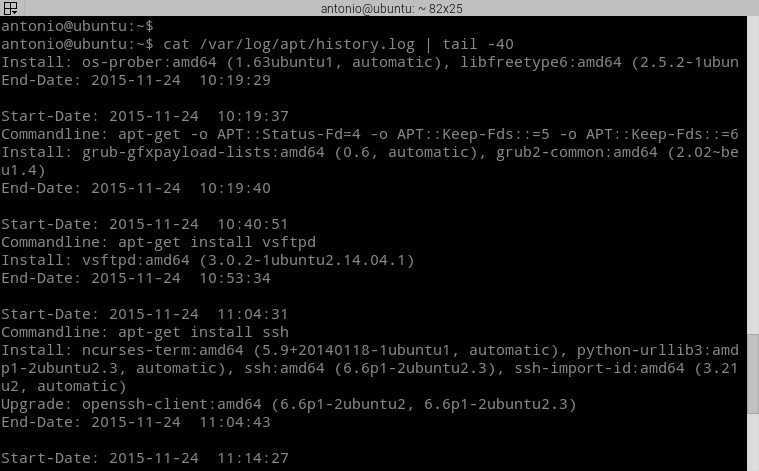
\includegraphics[width=\textwidth]{imagenes/logu}
        \caption{Log dpkg Ubuntu.}
    \end{subfigure}
    \begin{subfigure}[b]{0.8\textwidth}
        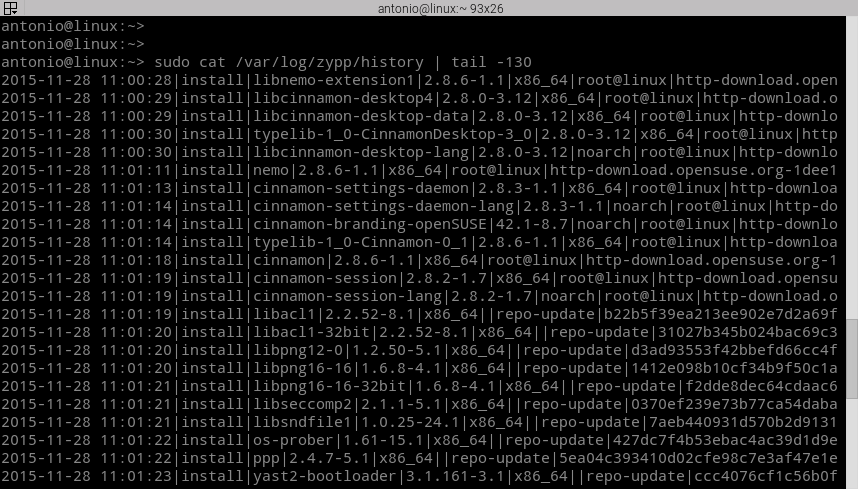
\includegraphics[width=\textwidth]{imagenes/logs}
        \caption{Log zypper OpenSuse.}
    \end{subfigure}
    \caption{Ejemplo historial de instalación.}
    \label{fig16}
\end{figure}

\begin{figure}[H]
  \begin{center}
    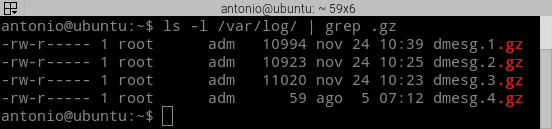
\includegraphics[width=1\textwidth]{imagenes/rot}
    \caption{En esta imagen se puede ver como los archivos con un numero más bajo en su nombre, se corresponden con fechas mas recientes.}
    \label{fig17}
  \end{center}
\end{figure}

\subsubsection{Cuestión opcional 1}
\textit{Indique qué comandos ha utilizado para realizarlo así como capturas de pantalla del proceso de reconstrucción del RAID.}
\newline

Para realizar esta cuestión, he simulado un fallo por software en el RAID y luego he monitorizado el proceso de reconstrucción. Para esto he realizado el mismo proceso que en la primera práctica, he simulado un fallo, luego he comprobado que el fallo se ha producido correctamente, y por último he retirado y añadido un nuevo disco, este proceso se puede ver en la \cref{fig18}\cite{fault}. Para la monitorización del proceso de reconstrucción se hecho uso de la orden indicada en el guión \texttt{watch -n2 cat /proc/mdstat}, esta orden se encarga de ejecutar un programa periódicamente y mostrarlo en pantalla\cite{watch}, en este caso ejecuta el comando cat cada dos segundos, lo que nos permite ver el como va evolucionando el proceso de reconstrucción del RAID, como se puede ver en \cref{fig19}.

\begin{figure}[H]
  \begin{center}
    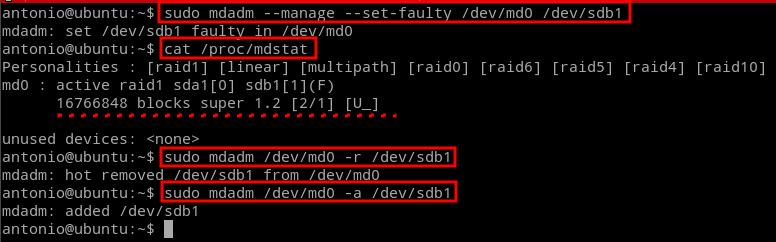
\includegraphics[width=1\textwidth]{imagenes/mdadm}
    \caption{Proceso para simular un fallo de disco, comprobarlo, eliminar el disco que ha fallado y añadir uno nuevo.}
    \label{fig18}
  \end{center}
\end{figure}

\begin{figure}[H]
  \begin{center}
    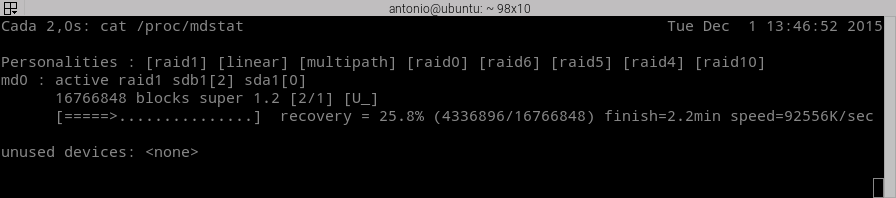
\includegraphics[width=1\textwidth]{imagenes/watch}
    \caption{Vista del proceso de reconstrucción haciendo uso de la orden watch.}
    \label{fig19}
  \end{center}
\end{figure}

\subsection{Programando tareas con CRON}
\subsubsection{Cuestión 2}
\textit{¿qué archivo ha de modificar para programar una tarea? Escriba la línea necesaria para ejecutar una vez al día una copia del directorio ~/codigo a ~/seguridad/\$fecha donde \$fecha es la fecha actual (puede usar el comando date).}
\newline

Para programar una tarea hay que modificar el archivo crontab \cite{cron} \cite{cron2}. Para ejecutar una orden que realice una vez al día la copia del directorio ~/codigo, se debería incluir una línea en el archivo crontab ( se puede realizar mediante el uso de la orden \texttt{crontab -e}) como la que se puede ver en la  \cref{fig1} \cite{date}.

\begin{figure}[H]
  \begin{center}
    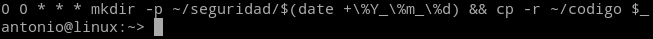
\includegraphics[width=1\textwidth]{imagenes/cron}
    \caption{Comando insertado en crontab para realizar una copia de seguridad diaria.}
    \label{fig1}
  \end{center}
\end{figure}

\subsection{Analizando qué ocurre en el kernel con DMESG}


\subsubsection{Cuestión 3}
\textit{Pruebe a ejecutar el comando, conectar un dispositivo USB y vuelva a ejecutar el comando. Copie y pegue la salida del comando. (considere usar dmesg | tail). Comente qué observa en la información mostrada.}
\newline

Al ejecutar el comando por primera vez obtenemos la información mostrada en la  \cref{fig2}, tras insertar un dispositivo USB, la información mostrada cambia como se muestra en la  \cref{fig3}. En esta información se muestran datos acerca del dispositivo USB conectado, entre los que se incluyen el nombre del producto, el fabricante y el numero de serie entre otros.
\begin{figure}[H]
  \begin{center}
    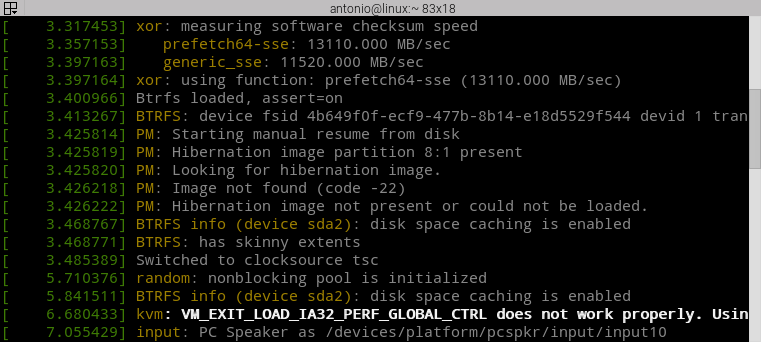
\includegraphics[width=1\textwidth]{imagenes/dmesg1}
    \caption{Ejecución de dmesg antes de insertar un USB.}
    \label{fig2}
  \end{center}
\end{figure}
\begin{figure}[H]
  \begin{center}
    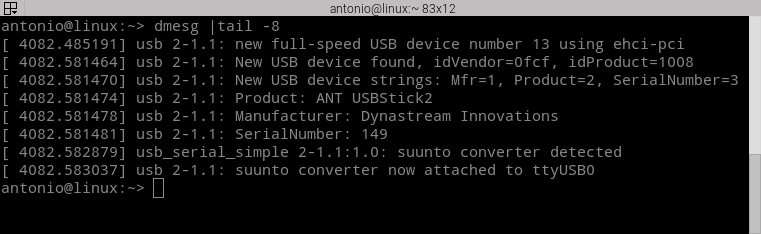
\includegraphics[width=1\textwidth]{imagenes/dmesg2}
    \caption{Ejecución de dmesg tras la conexión de un dispositivo USB, con información acerca de dispositivo conectado.}
    \label{fig3}
  \end{center}
\end{figure}

\section{Monitorizando Windows: PERFMON}
\subsection{Cuestión 4}
\textit{Ejecute el monitor de ``System Performance'' y muestre el resultado. Incluya capturas de pantalla comentando la información que aparece.}
\newline

Para usar el monitor ``System Performance'' debemos abrir una consola y escribir la orden \texttt{perfmon} con lo que se obtiene una pantalla como la mostrada en la  \cref{fig4}, en la que aparecen varias cosas: a la izquierda, tenemos un menú para realizar diferentes tareas con el monitor, en la parte central de la pantalla aparecen tres cuadros, dos de ellos para obtener información y uno con un resumen del sistema en el que se muestran estadísticas sobre el disco duro, el procesador,la red y la memoria RAM. Para acceder a el monitor ``System Performance'' debemos dirigirnos al lado izquierdo y pinchar en ``Conjunto de  recopiladores de datos'' , ``Sistema'' y ``System Performance''. Una vez ahí procedemos a iniciar el conjunto de recopiladores de datos durante un tiempo, luego nos dirigimos a apartado ``Informes'' , ``Sistema'' y ``System Performance'' y ya podemos ver el conjunto de datos recopilados como se muestra en la \cref{fig29}.

\begin{figure}[H]
  \begin{center}
    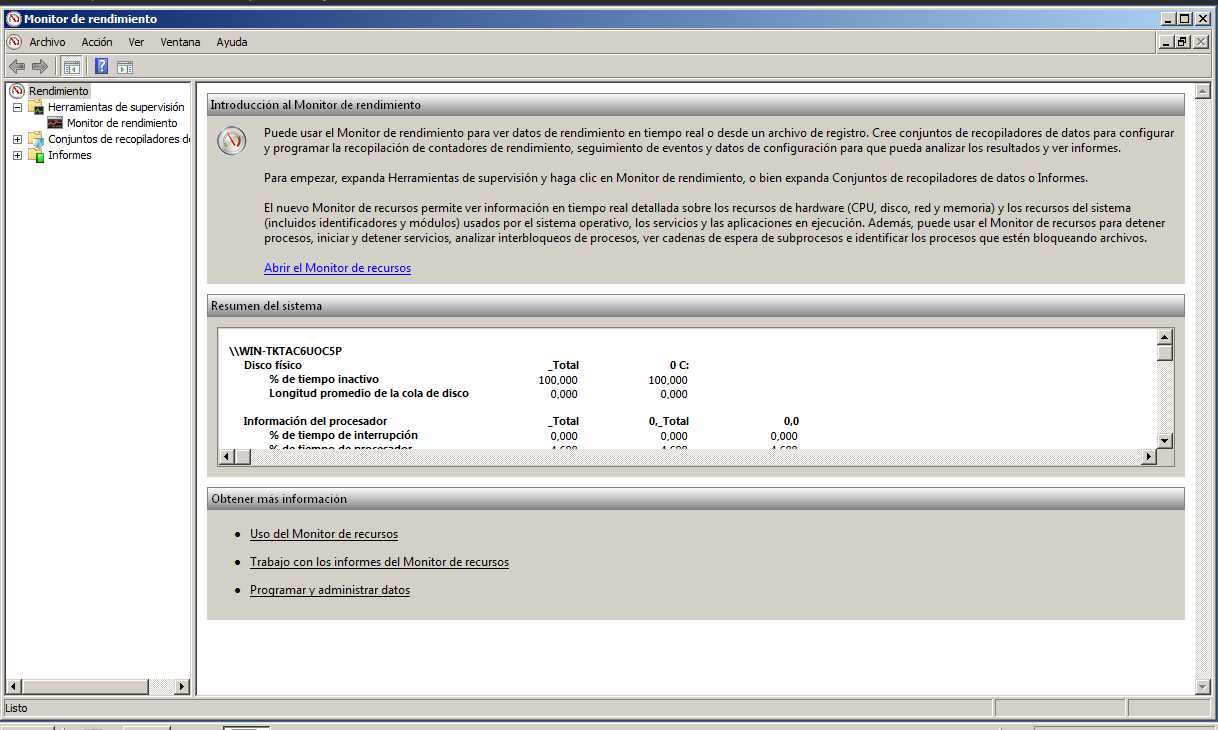
\includegraphics[width=0.8\textwidth]{imagenes/perfmon}
    \caption{Pantalla inicial de ``System Performance''.}
    \label{fig4}
  \end{center}
\end{figure}

\begin{figure}[H]
  \begin{center}
    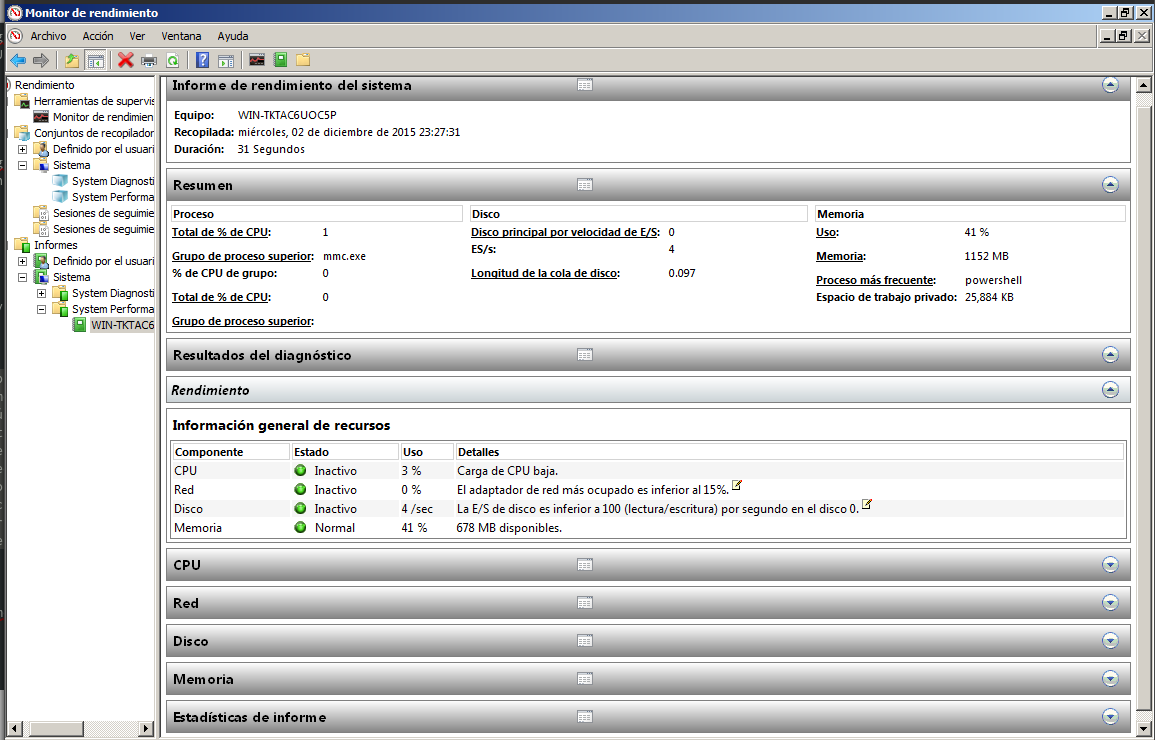
\includegraphics[width=0.8\textwidth]{imagenes/perfmon2}
    \caption{Resultado de la ejecución de ``System Performance'', en la que se puede ver un resumen de los datos recopilados ( uso de memoria, longitud de la cola del disco ,total de \% de CPU...) y la existencia de varios apartados en los que se proporciona gran cantidad de datos.}
    \label{fig29}
  \end{center}
\end{figure}

\subsection{Cuestión 5}
\textit{Cree un recopilador de datos definido por el usuario (modo avanzado) que incluya tanto el contador de rendimiento como los datos de seguimiento:Todos los referentes al procesador, al proceso y al servicio web. Intervalo de muestra 15 segundos. Almacene el resultado en el directorio Escritorio\\logs Incluya las capturas de pantalla de cada paso.}
\newline

El proceso para la creación de un recopilador de datos con las características citadas en la cuestión, se puede ver en en las \crefrange{fig5}{fig12}.

\begin{figure}[H]
  \begin{center}
    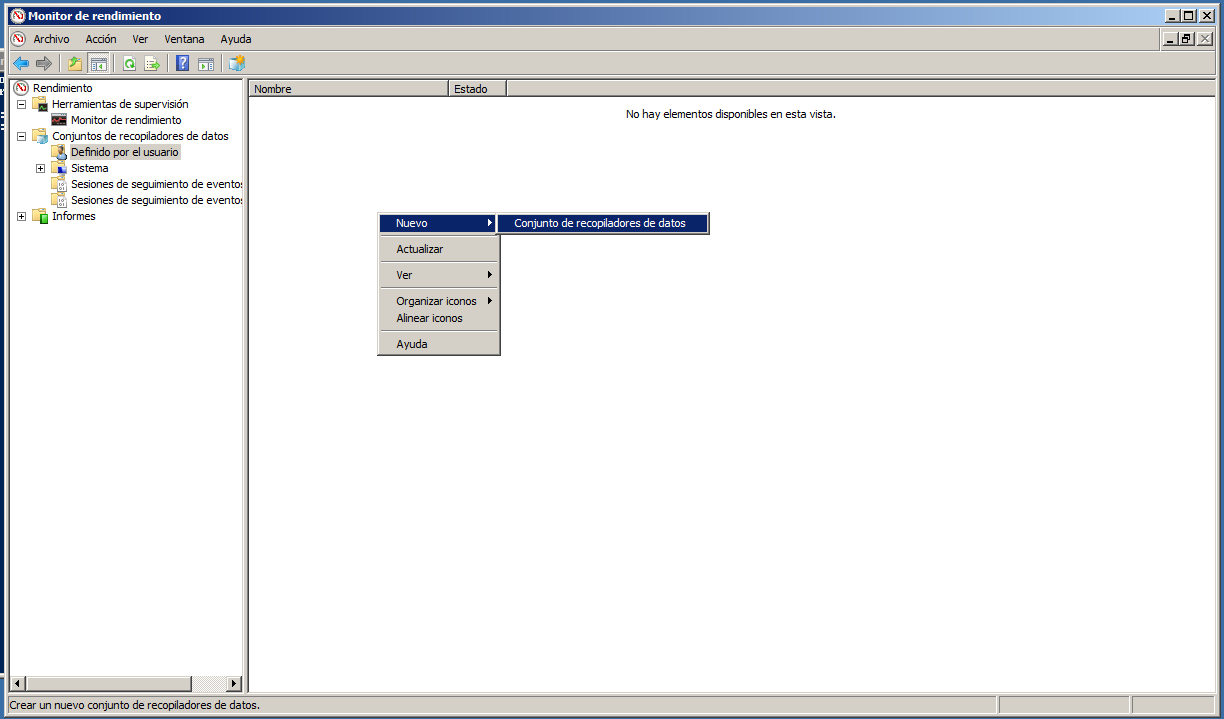
\includegraphics[width=1\textwidth]{imagenes/rec1}
    \caption{Panatalla para empezar a crear un nuevo recopilador.}
    \label{fig5}
  \end{center}
\end{figure}

\begin{figure}[H]
  \begin{center}
    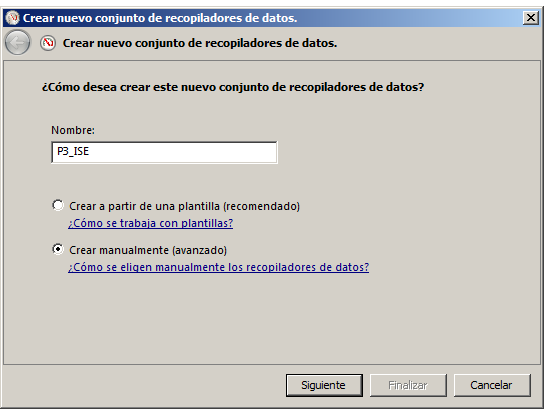
\includegraphics[width=0.7\textwidth]{imagenes/rec2}
    \caption{Selección del nombre y la forma de creación del recopilador''.}
    \label{fig6}
  \end{center}
\end{figure}

\begin{figure}[H]
  \begin{center}
    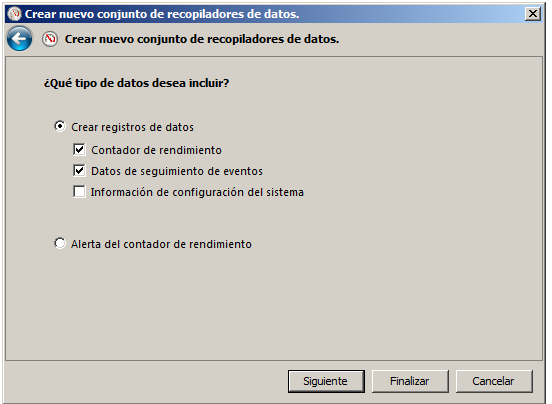
\includegraphics[width=0.7\textwidth]{imagenes/rec3}
    \caption{Pantalla para seleccionar que datos se desean incluir.}
    \label{fig7}
  \end{center}
\end{figure}

\begin{figure}[H]
  \begin{center}
    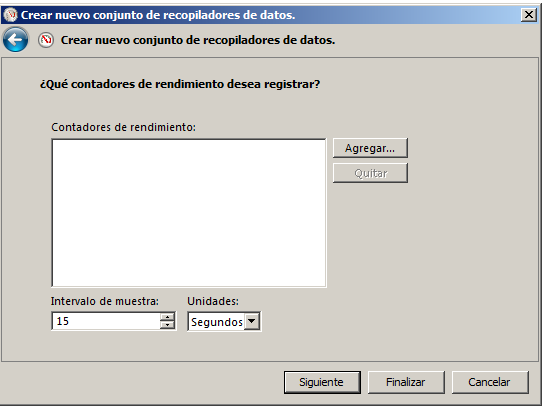
\includegraphics[width=0.7\textwidth]{imagenes/rec3_5}
    \caption{Pantalla para agregar contadores de rendimiento}
    \label{fig8}
  \end{center}
\end{figure}

\begin{figure}[H]
  \begin{center}
    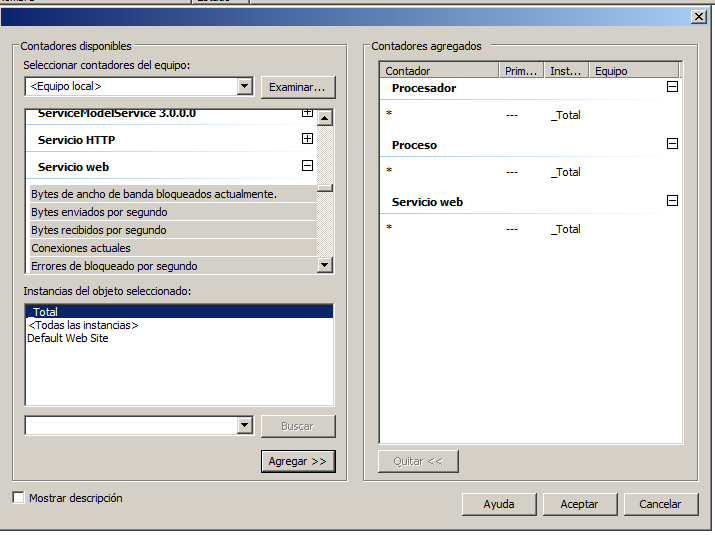
\includegraphics[width=0.7\textwidth]{imagenes/rec4}
    \caption{Proceso para seleccionar los contadores de rendimiento que se quieren añadir.}
    \label{fig9}
  \end{center}
\end{figure}

\begin{figure}[H]
  \begin{center}
    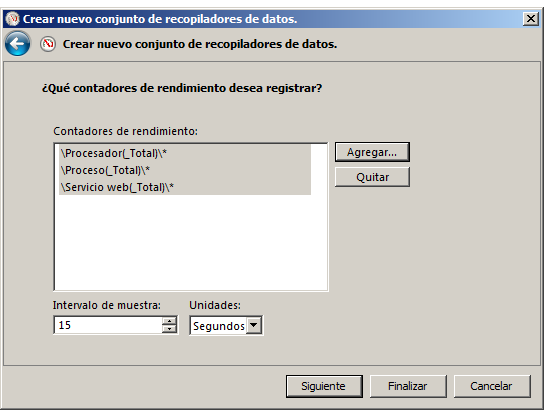
\includegraphics[width=0.7\textwidth]{imagenes/rec5}
    \caption{Pantalla con los contadores de rendimiento seleccionados.}
    \label{fig10}
  \end{center}
\end{figure}

\begin{figure}[H]
  \begin{center}
    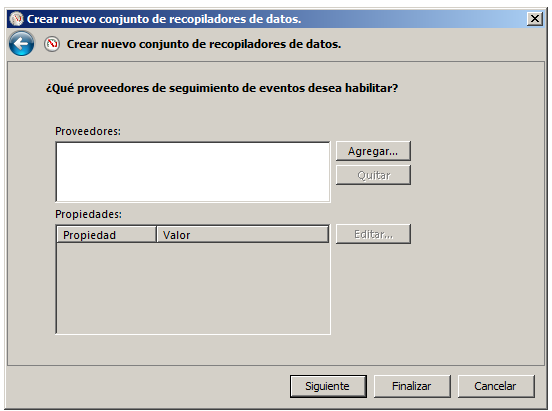
\includegraphics[width=0.7\textwidth]{imagenes/rec6}
    \caption{Pantalla para seleccionar proveedores de seguimiento.}
    \label{fig11}
  \end{center}
\end{figure}

\begin{figure}[H]
  \begin{center}
    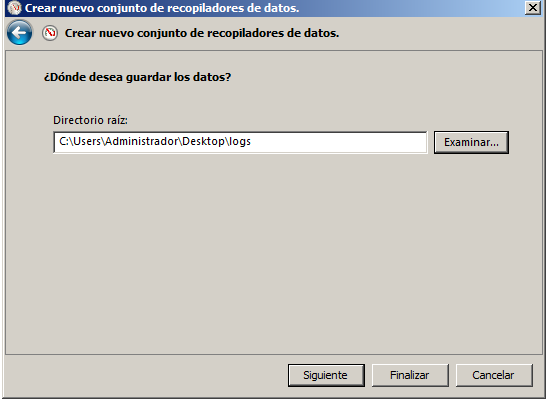
\includegraphics[width=0.7\textwidth]{imagenes/rec7}
    \caption{Pantalla para indicar la ruta donde se guardaran los datos.}
    \label{fig12}
  \end{center}
\end{figure}



\section{Monitorizando el hardware}
\subsection{Cuestión 6}
\textit{Instale alguno de los monitores comentados arriba en su máquina y pruebe a ejecutarlos (tenga en cuenta que si lo hace en la máquina virtual, los resultados pueden no ser realistas). Alternativamente, busque otros monitores para hardware comerciales o de código abierto para Windows y Linux.}
\newline

Para este apartado he instalado los monitores lm-sensors y hddtemp, usando el comando mostrado en la \cref{fig13}. Los resultados de la ejecución muestran datos sobre la temperatura y los voltajes, como se muestra en las \crefrange{fig14}{fig15}.

\begin{figure}[H]
  \begin{center}
    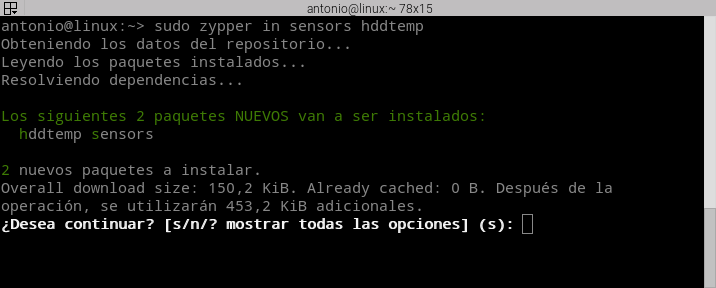
\includegraphics[width=1\textwidth]{imagenes/sensors}
    \caption{Instalación de los monitores hddtemp y lm-sensors en OpenSuse.}
    \label{fig13}
  \end{center}
\end{figure}

\begin{figure}[H]
    \centering
    \begin{subfigure}[b]{0.75\textwidth}
        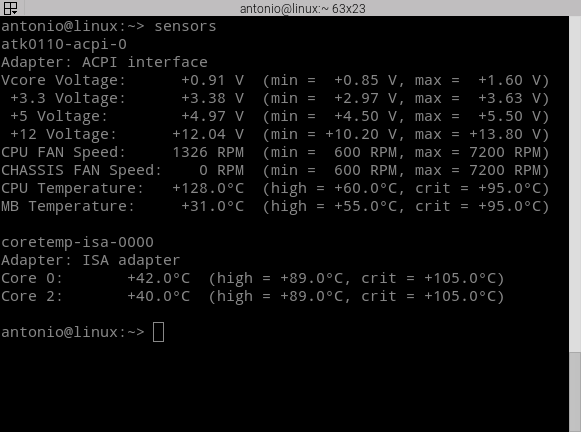
\includegraphics[width=\textwidth]{imagenes/sensors2}
        \caption{Ejecución de lm-sensors.}
        \label{fig14}
    \end{subfigure}
    \begin{subfigure}[b]{0.75\textwidth}
        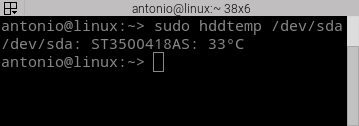
\includegraphics[width=\textwidth]{imagenes/hddtemp}
        \caption{Ejecución de hddtemp.}
        \label{fig15}
    \end{subfigure}
    \caption{Ejecución monitores lm-sensors y hddtemp.}
\end{figure}

\section{Otros monitores del sistema}
\subsection{MUNIM}
\subsubsection{Cuestión 7}
\textit{Visite la web del proyecto y acceda a la demo que proporcionan (\url{http://demo.munin-monitoring.org/}) donde se muestra cómo monitorizan un servidor. Monitorice varios parámetros y haga capturas de pantalla de lo que está mostrando comentando qué observa.}
\newline

Al acceder a \url{http://demo.munin-monitoring.org/} nos encontramos con una web como la mostrada en la \cref{fig40}, en esta pantalla nos encontramos con gran cantidad de opciones, cada una de ellas nos permite monitorizar alguna parte de nuestro servidor, como puede ser el uso de memoria, el uso de disco, el uso de CPU, el numero de procesos, ademas nos permite monitorizar servicios del servidor como VPN o Apache. Para ver algún ejemplo de las gráficas proporcionadas me he dirigido al apartado y me he centrado en el numero de threads, como se puede ver en \cref{fig41}, donde se ofrece una breve descripción de los gráficos mostrados.

\begin{figure}[H]
  \begin{center}
    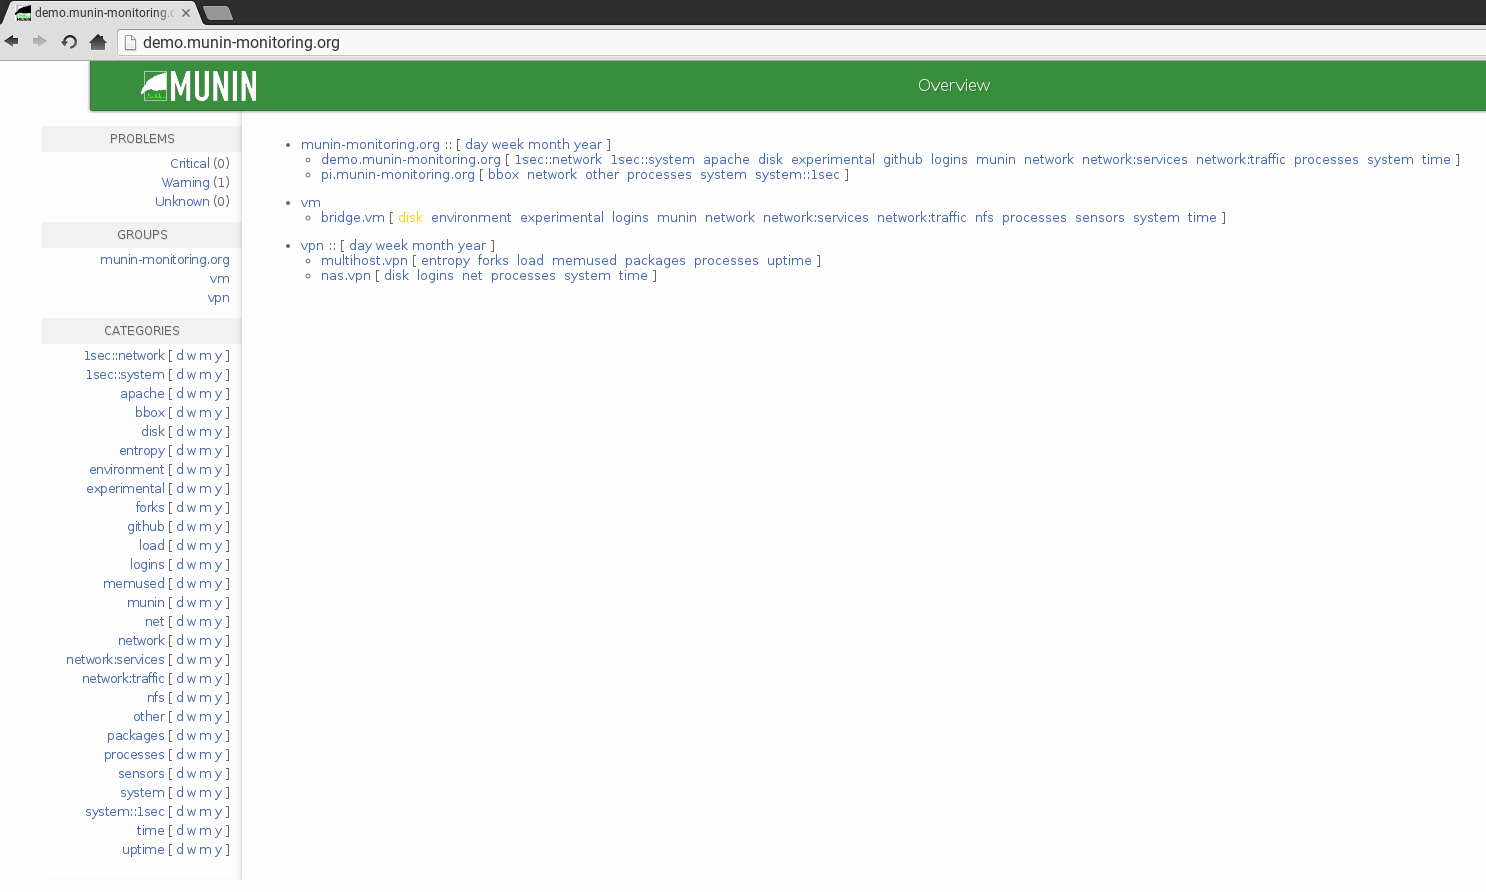
\includegraphics[width=1\textwidth]{imagenes/mun1}
    \caption{En esta imagen se muestra la pantalla inicial de la demo de Munin.}
    \label{fig40}
  \end{center}
\end{figure}

\begin{figure}[H]
  \begin{center}
    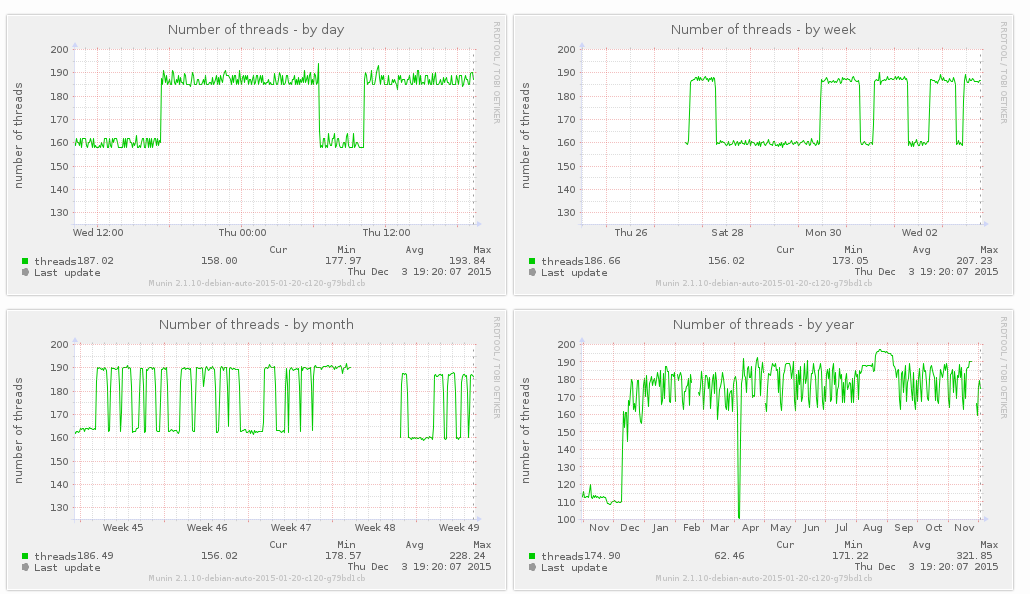
\includegraphics[width=1\textwidth]{imagenes/mun2}
    \caption{En esta gráfica se muestra el numero de threads que se están ejecutando en el servido, con lo que podemos ver algunas cosas que pueden ser útiles para el administrador de un servidor, por ejemplo al ver la gráfica semana y mensual, se puede observar que la carga que tiene el servidor los fines de semanas es menor que los días laborales, además en la primera gráfica podemos ver en que horas el servidor tiene mas carga de tareas.}
    \label{fig41}
  \end{center}
\end{figure}


\subsection{ZABBIX}
\subsubsection{Cuestión opcional 4}
\textit{Prueba a instalar este monitor es alguno de sus tres sistemas. Realice capturas de pantalla del proceso de instalación y comente capturas de pantalla del programa en ejecución.}
En esta cuestión he llevado a cabo la instalación y configuración de Zabbix en Ubuntu Server, el proceso se muestra en las \crefrange{fig30}{fig35} \cite{zab}

\begin{figure}[H]
  \begin{center}
    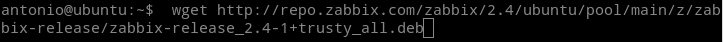
\includegraphics[width=1\textwidth]{imagenes/zab1}
    \caption{Descarga del repositorio de Zabbix.}
    \label{fig30}
  \end{center}
\end{figure}

\begin{figure}[H]
  \begin{center}
    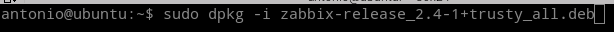
\includegraphics[width=1\textwidth]{imagenes/zab2}
    \caption{Instalación del paquete descargado en \cref{fig30}.}
    \label{fig31}
  \end{center}
\end{figure}

\begin{figure}[H]
  \begin{center}
    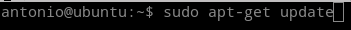
\includegraphics[width=0.6\textwidth]{imagenes/zab3}
    \caption{Actualización de los paquetes disponibles.}
    \label{fig32}
  \end{center}
\end{figure}

\begin{figure}[H]
  \begin{center}
    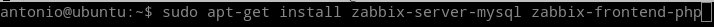
\includegraphics[width=1\textwidth]{imagenes/zab4}
    \caption{Instalación de Zabbix y sus requisitos.}
    \label{fig33}
  \end{center}
\end{figure}

\begin{figure}[H]
  \begin{center}
    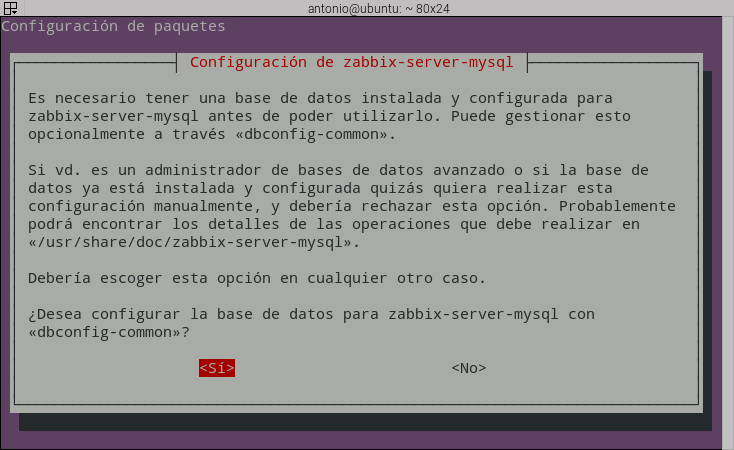
\includegraphics[width=0.75\textwidth]{imagenes/zab5}
    \caption{Configurcion de una base de datos para Zabbix.}
    \label{fig34}
  \end{center}
\end{figure}

\begin{figure}[H]
  \begin{center}
    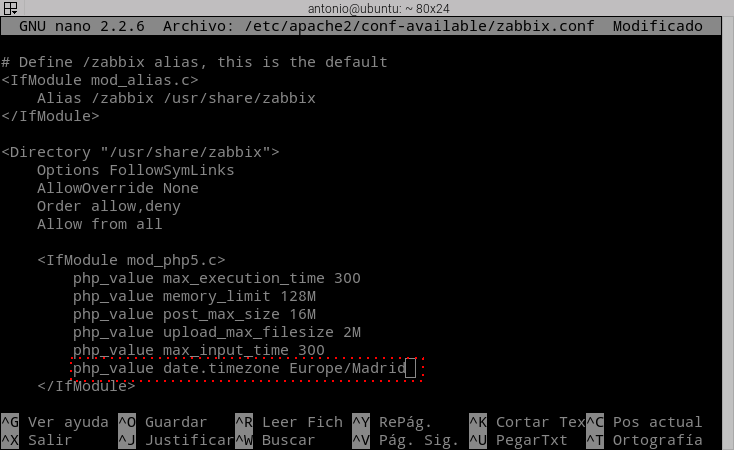
\includegraphics[width=0.75\textwidth]{imagenes/zab6}
    \caption{Configuración obligatoria de la zona horaria de Zabbix en el archivo \texttt{/etc/apache2/conf-avaible/Zabbix.conf}.}
    \label{fig35}
  \end{center}
\end{figure}

Tras esto, accedemos a Zabbix mediante un navegador web haciendo uso de la IP de nuestro servidor ( 192.168.56.101/Zabbix ) y nos aparecerá un asistente de configuración ( \cref{fig36} ) en el que deberemos introducir nuestra contraseña y nuestra IP en lugar de localhost, una vez realizado esto debemos instalar Zabbix-agent ( \cref{fig37} ), que es el proceso que se encargara de mandar la información del servidor al servidor de Zabbix ( en este caso son la misma máquina por lo que no hay que modificar la configuración de Zabbix-agent donde se indica la IP del servidor). Por último entramos en 192.168.56.101/Zabbix y accedemos con el usuario ``Admin'' y la contraseña ``Zabbix''. Una vez dentro nos dirigimos al apartado Configuration/Host y habilitamos el servidor que queremos monitorizar ( \cref{fig38} ). Con esto lo tenemos todo funcionando y ya podemos monitorizar nuestro servidor mediante las diferentes opciones que el Zabbix ofrece como el uso de gráficas mostrado en la (\cref{fig39}).   

\begin{figure}[H]
  \begin{center}
    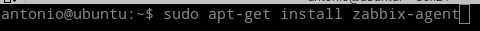
\includegraphics[width=1\textwidth]{imagenes/zab9}
    \caption{Instalación de Zabbix-agent.}
    \label{fig36}
  \end{center}
\end{figure}

\begin{figure}[H]
  \begin{center}
    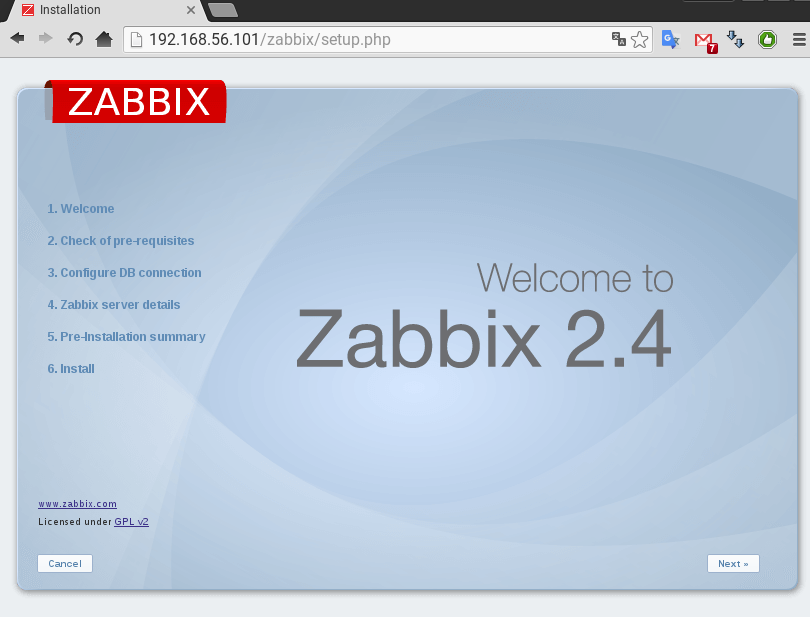
\includegraphics[width=1\textwidth]{imagenes/asist}
    \caption{Asistente de configuración Zabbix.}
    \label{fig37}
  \end{center}
\end{figure}

\begin{figure}[H]
  \begin{center}
    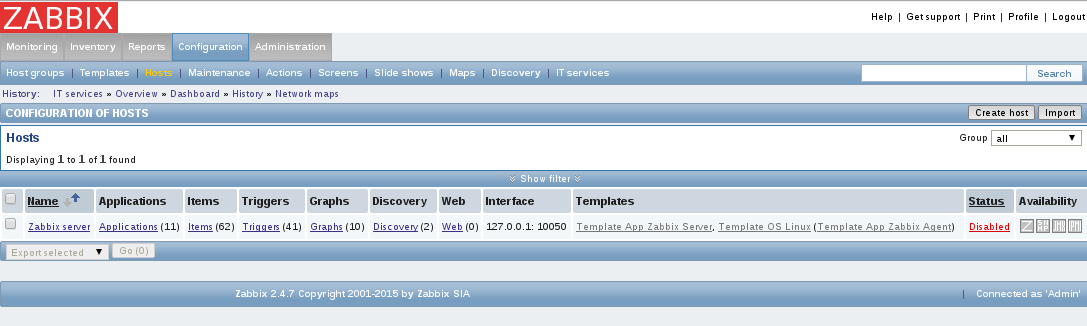
\includegraphics[width=1\textwidth]{imagenes/enable}
    \caption{Activación de la monitorización.}
    \label{fig38}
  \end{center}
\end{figure}


\begin{figure}[H] 
  \begin{subfigure}[b]{0.5\linewidth}
    \centering
    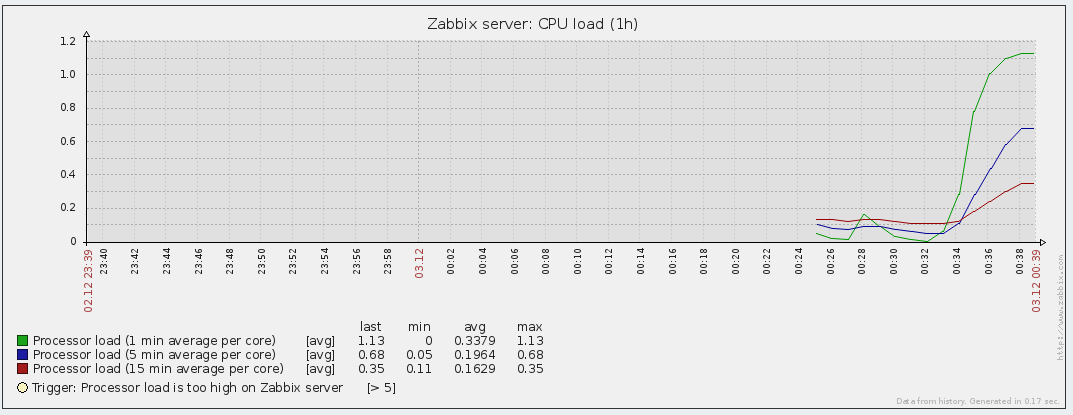
\includegraphics[width=0.95\linewidth]{imagenes/g1} 
    \caption{Gráfica de la carga de la CPU.} 
    \vspace{4ex}
  \end{subfigure}%% 
  \begin{subfigure}[b]{0.5\linewidth}
    \centering
    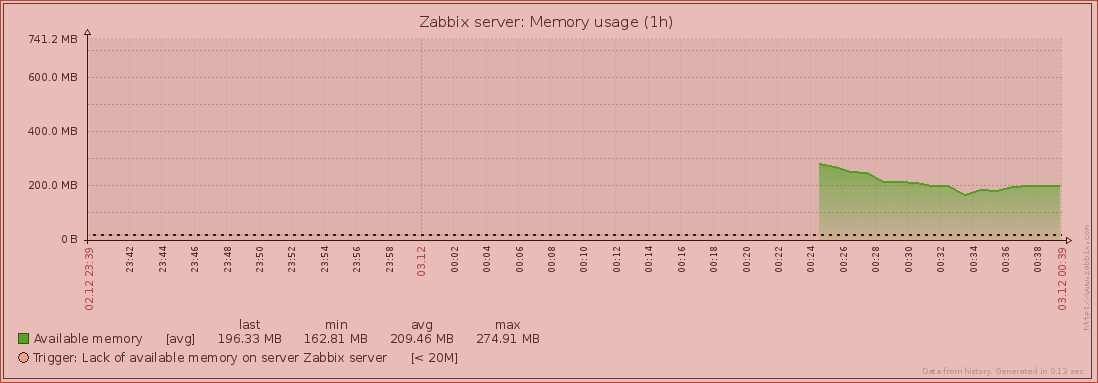
\includegraphics[width=0.95\linewidth]{imagenes/g2} 
    \caption{Gráfica de uso de memoria.} 
    \vspace{4ex}
  \end{subfigure} 
  \begin{subfigure}[b]{0.5\linewidth}
    \centering
    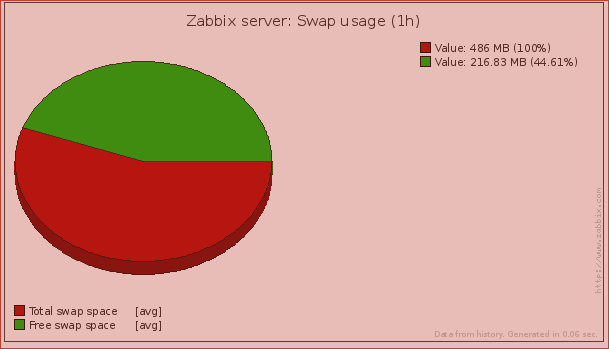
\includegraphics[width=0.95\linewidth]{imagenes/g3} 
    \caption{Gráfica del uso de swap.} 
  \end{subfigure}%%
  \begin{subfigure}[b]{0.5\linewidth}
    \centering
    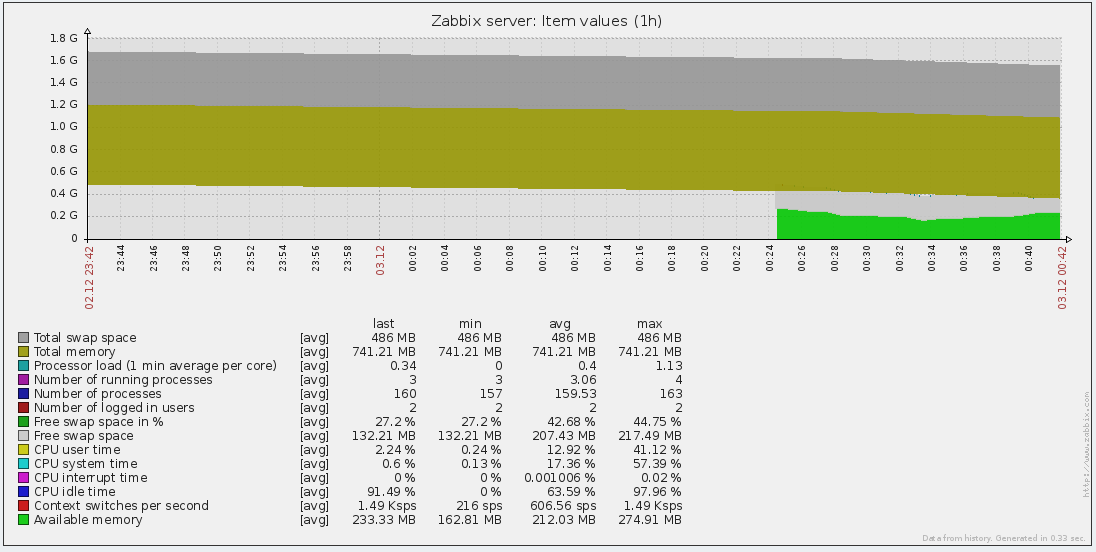
\includegraphics[width=0.95\linewidth]{imagenes/g4} 
    \caption{Gráfica personalizada con diversos parámetros de monitorización.} 
  \end{subfigure} 
  \caption{Algunas de las gráficas disponibles en Zabbix. }
  \label{fig39} 
\end{figure}


\subsection{AWSTATS}
\subsubsection{Cuestión opcional 6}
\textit{Instale el monitor y muestre y comente algunas capturas de pantalla.}

Para realizar esta cuestión me he apoyado en el manual disponible en \cite{aws}. Los pasos para la instalación, están explicados en las \crefrange{fig42}{fig43}.
\begin{figure}[H]
  \begin{center}
    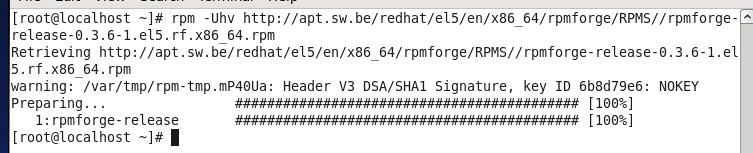
\includegraphics[width=1\textwidth]{imagenes/aw1}
    \caption{En esta figura añadimos el repositorio RPMForge a yum.}
    \label{fig42}
  \end{center}
\end{figure}
\begin{figure}[H]
  \begin{center}
    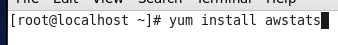
\includegraphics[width=1\textwidth]{imagenes/aw2}
    \caption{Tras ejecutar \texttt{yum update} procedemos a instalar AWStats con el comando indicado.}
    \label{fig43}
  \end{center}
\end{figure}
\begin{figure}[H]
  \begin{center}
    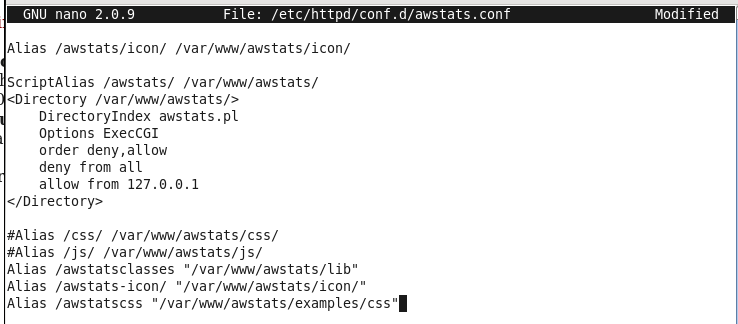
\includegraphics[width=1\textwidth]{imagenes/aw3}
    \caption{Una vez AWStats esta instalado, editamos en archivo\newline\texttt{ /etc/httpd/conf.d/awstats.conf} añadiendo las tres ultimas líneas.}
    \label{fig44}
  \end{center}
\end{figure}
\begin{figure}[H]
  \begin{center}
    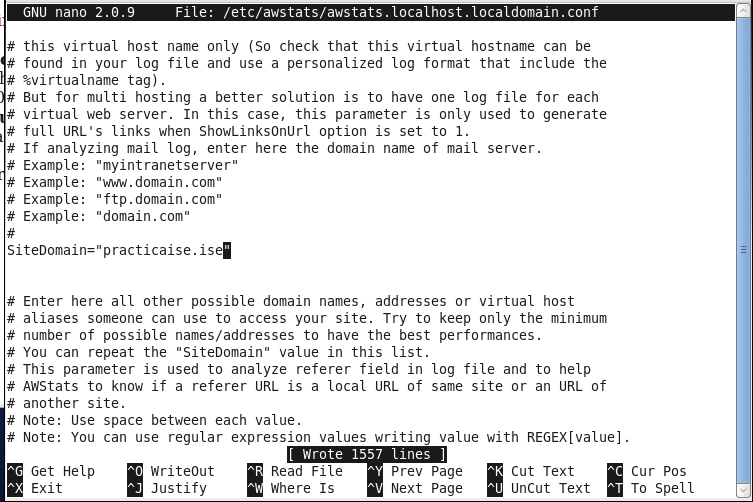
\includegraphics[width=1\textwidth]{imagenes/aw4}
    \caption{En esta imagen se muestra la edición que hay que realizar en \newline\texttt{/etc/awstats/awstats.localhost.localdomain.conf} (añadir un nombre a SiteDomain).}
    \label{fig45}
  \end{center}
\end{figure}
\begin{figure}[H]
  \begin{center}
    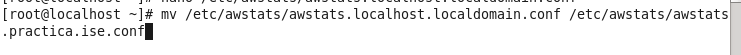
\includegraphics[width=1\textwidth]{imagenes/aw5}
    \caption{En este paso se mueve el archivo anteriormente a otro en el que se indica el nombre que pusimos en SiteDomain.}
    \label{fig46}
  \end{center}
\end{figure}
\begin{figure}[H]
  \begin{center}
    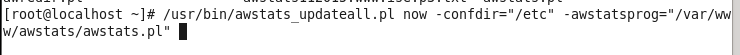
\includegraphics[width=1\textwidth]{imagenes/aw6}
    \caption{Por último ejecutamos el comando mostrado en la figura,para actualizar las estadísticas del servidor sin tener que esperar a que se actualicen solas..}
    \label{fig47}
  \end{center}
\end{figure}
\begin{figure}[H]
  \begin{center}
    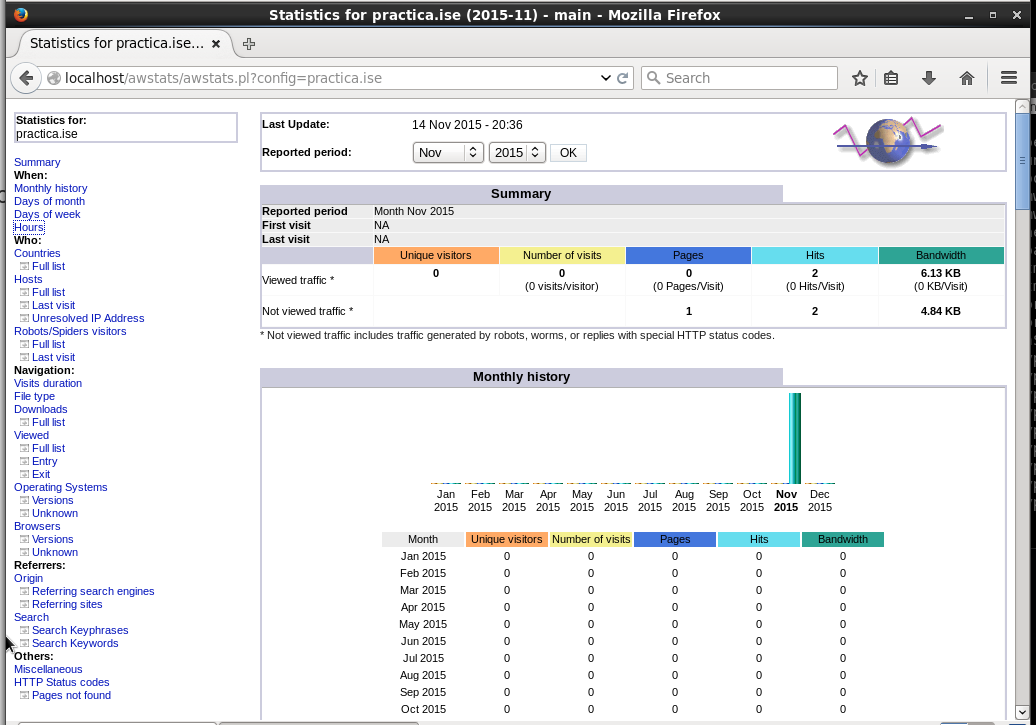
\includegraphics[width=1\textwidth]{imagenes/aw7}
    \caption{En este paso accedemos a la URL que aparece en la imagen para verificar que AWStats esta funcionando correctamente con lo que obtenemos la pagina inicial de AWStats con un resumen de las estadísticas de nuestro caso, en este caso no hay mucha información, ya que AWStats esta recién instalado (solo se muestra que ha habido 2 hits (peticiones de archivos que ha realizado el visitante \cite{aws2}).}
    \label{fig48}
  \end{center}
\end{figure}
\subsection{Monitorizando un servicio (o ejecución de un programa)}
\subsubsection{Cuestión 8}
\textit{Escriba un breve resumen sobre alguno de los artículos donde se muestra el uso de strace o busque otro y coméntelo.}
\newline

Para esta cuestión he usado el primer articulo \cite{fw}.En el Chad Fowler comienza haciendo una introducción en la que explica que gracias a la herramienta de UNIX strace, pudo solucionar un problema que tenia con un servidor con Lotus Domino que usaba UNIX. Tras esta, se explica que es strace. 


Strace es una herramienta de la línea de comandos que permite seguir las llamadas al sistema y las señales recibidas por un proceso en concreto y sus hijos. Tras dar una breve explicación de que es strace, el autor procede a hacer un demostración con un programa en C muy sencillo ( como el típico Hola Mundo ) y muestra la salida producida por la orden \texttt{strace -s 2000 -f ./traceme}, los parámetros pasados a strace significan: \texttt{-s 2000} sirve para indicar el tamaño máximo de los string que se quieren imprimir y \texttt{-f} se usa para indicar que se sigan todos los hijos del programa pasado como argumento. Después en los a partir del párrafo cuatro hasta el final de la sección, se explican algunas de las cosas que se muestran en la salida, como \texttt{execve(), write() y mmap() }.

Tras esta introducción se muestra el uso de strace sobre un proceso real que ya se esta ejecutando, en este apartado para poder conectar con un proceso que ya se esta ejecutando se hace uso de \texttt{-p pid} y ademas se añade la opción \texttt{-o} para indicar donde queremos guardar la salida de strace, ya que al ser un proceso real la salida será demasiado grande como para verla en la terminal, y ademas se muestra que para dejar de seguir al proceso se hace uso de \texttt{Ctrl+C}. Una vez ejecutado strace sobre el proceso se vuelve a dar una explicación sobre lo que se muestra, y se comentan nuevos datos como \texttt{select(), fstat(),recvfrom()}, la utilidad de \texttt{-e raw=} y el comando \texttt{lsof}, tras esto haciendo uso de las cosas nombradas anteriormente y algunas mas se sacan algunas conclusiones sobre el funcionamiento del programa que se esta examinando, por ejemplo que \texttt{accept4()} tiene un devuelve numero relativamente alto de fallos y que el proceso pasa la mayor parte del tiempo esperando algo ( la mayor parte del tiempo es consumida por \texttt{select()}, que se usa para esperar conexiones. 
Tras esta sección se explica como usar strace para averiguar que es lo que provoca los problemas de rendimiento en nuestro sistema, para explicar esto se hace uso de un programa en C muy simple y se ejecuta con strace haciendo uso de la opción \texttt{-T} que sirve para que se muestre el tiempo de cada llamada al sistema y explica que en la vida real podríamos guardar la salida y ordenarla para encontrar las llamadas mas lentas. 


Para finalizar el autor menciona que existen más casos en los que se puede usar strace y en relación al problema inicial, dice que consiguieron solucionar el problema del servidor Lotus Domino.

\section{Profiling}

\subsection{PYTHON}
\subsubsection{Cuestión opcional 9}
\textit{Escriba un script en python y analice su comportamiento usando el profiler presentado.}
\newline

Para probar el profiler de python cProfile \cite{cprofile}, he creado un script que lee un archivo con gran cantidad de números y luego comprueba cuales son primos y los guarda en otro archivo ( \cref{fig20} ). Tras la ejecución del script con el profiler, se muestra una tabla ( \cref{fig21} ) en la que se muestra información sobre el tiempo y el numero de llamadas que ha consumido cada función. En el caso de mi script se puede ver que la función que mas tiempo a consumido es la que comprueba si los números son primos.
\newline

El significado de las diferentes columnas es \cite{cprofile}:
\begin{enumerate}
  \item \textbf{ncalls:} Es el número de llamadas que se han realizado a una función.
  \item \textbf{tottime:} Es el tiempo que ha requerido una función, sin contar el tiempo consumido en llamadas a subfunciones.
  \item \textbf{percall:} Es el tiempo por llamada, es decir tottime dividido entre ncalls.
  \item \textbf{cumtime:} Es el tiempo que ha consumido una función incluyendo el tiempo consumido por las subfunciones.
  \item \textbf{percall:} Es el tiempo cumtime dividido entre las llamadas primitivas (primitive calls).
  \item \textbf{filename:lineno(function):} Da una descripción de la llamada.
\end{enumerate}

\begin{figure}[H]
  \begin{center}
    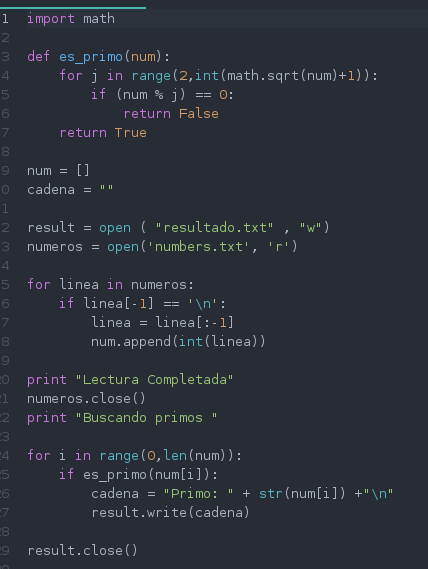
\includegraphics[width=1\textwidth]{imagenes/primo}
    \caption{Código del script que busca los números primos.}
    \label{fig20}
  \end{center}
\end{figure}

\begin{figure}[H]
  \begin{center}
    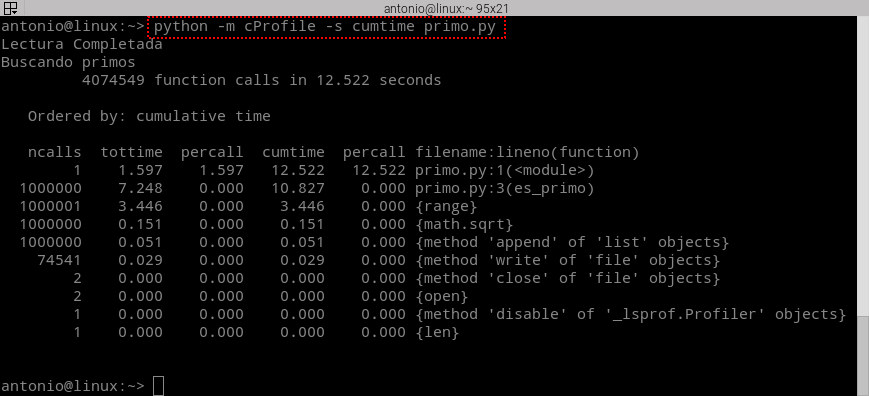
\includegraphics[width=1\textwidth]{imagenes/cprof}
    \caption{En esta imagen se muestrta el resultado de cProfile. La orden \texttt{-s cumtime} pasada a cProfile, indica que las filas deben estar ordenadas según el tiempo acumulativo, es decir el tiempo que ha requerido la función mas todas las subfunciones a las que esta invoque. }
    \label{fig21}
  \end{center}
\end{figure}


\subsubsection{Cuestión 9}
\textit{Acceda a la consola MySQL (o a través de phpMyAdmin) y muestre el resultado de mostrar el ''profile'' de una consulta (la creación de la BD y la consulta la puede hacer líbremente).}
\newline

Para realizar esta cuestión he descargado una base de datos de ejemplo \cite{db}( con aproximadamente 300000 empleado y 2,8 millones entradas sobre salarios ), que tiene la estructura indicada en \cite{db1} y esta disponible para la descarga en \url{https://launchpad.net/test-db/} luego la he importado haciendo siguiendo los pasos mostrado en las \crefrange{fig22}{fig24}.

Para probar el profile primero lo he habilitado como se puede ver en \cref{fig25}, luego he realizado un consulta buscando que empleados cobran más de 155000\euro como se puede ver en \cref{fig26} y por último he mirado los resultados de la consulta haciendo uso de \texttt{SHOW PROFILES}( \cref{fig27}) y \texttt{SHOW PROFILE}(\cref{fig28}). \texttt{SHOW PROFILES} se muestra una lista de las consultas que se han realizado más recientemente y \texttt{SHOW PROFILE}muestra datos detallados de una consulta especifica realizada, como pueden ser los bloques de entrada y salida, el uso de CPU y los cambios de contexto entre otros. En el ejemplo de (\cref{fig28}) solo se muestra información sobre el tiempo empleado y el uso de CPU. \cite{db2}

\begin{figure}[H]
  \begin{center}
    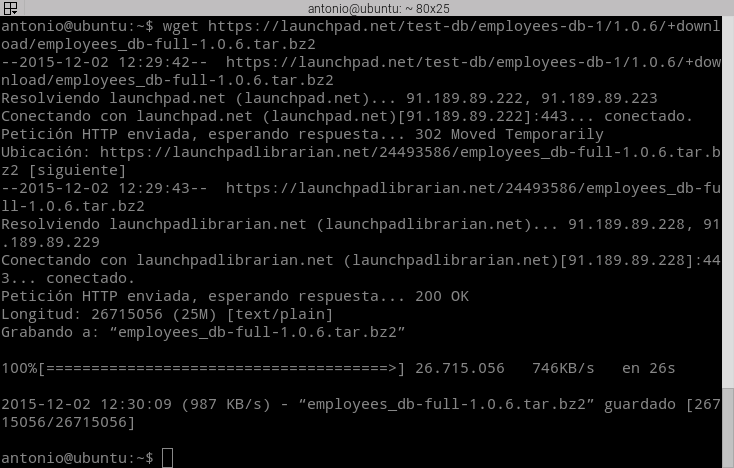
\includegraphics[width=1\textwidth]{imagenes/descarga}
    \caption{Orden para la descarga de la base de datos de ejemplo.}
    \label{fig22}
  \end{center}
\end{figure}

\begin{figure}[H]
  \begin{center}
    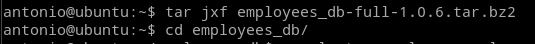
\includegraphics[width=1\textwidth]{imagenes/extraccion}
    \caption{Orden para extraer el archivo descargado.}
    \label{fig23}
  \end{center}
\end{figure}

\begin{figure}[H]
  \begin{center}
    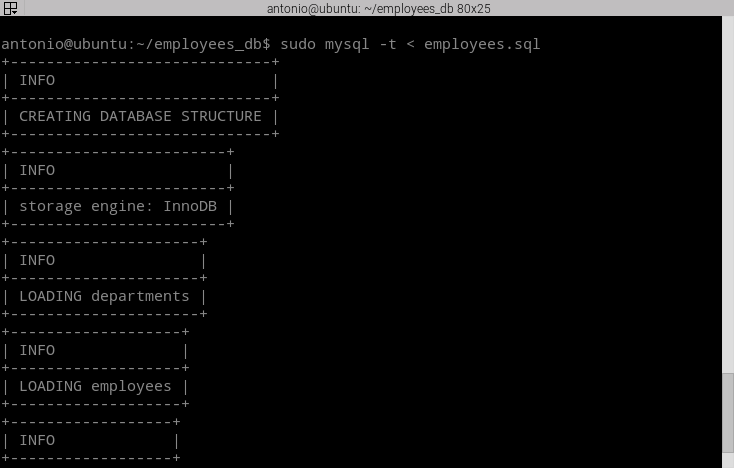
\includegraphics[width=1\textwidth]{imagenes/importacion}
    \caption{Proceso para importar desde MySQL la base de datos descargada.}
    \label{fig24}
  \end{center}
\end{figure}

\begin{figure}[H]
  \begin{center}
    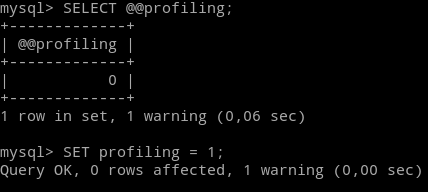
\includegraphics[width=1\textwidth]{imagenes/prof}
    \caption{Activación del profiler.}
    \label{fig25}
  \end{center}
\end{figure}

\begin{figure}[H]
  \begin{center}
    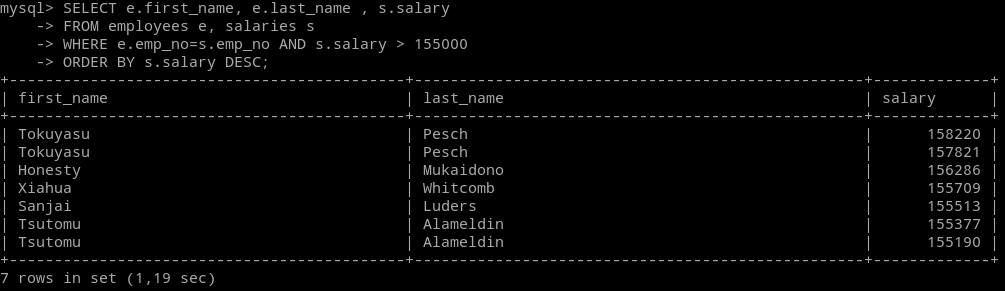
\includegraphics[width=1\textwidth]{imagenes/consulta}
    \caption{Consulta SQL.}
    \label{fig26}
  \end{center}
\end{figure}

\begin{figure}[H]
  \begin{center}
    \includegraphics[width=1\textwidth]{imagenes/profs}
    \caption{Resultado de ejecutar \texttt{SHOW PROFILES}.}
    \label{fig27}
  \end{center}
\end{figure}

\begin{figure}[H]
  \begin{center}
    \includegraphics[width=1\textwidth]{imagenes/mpr}
    \caption{Resultado de la ejecución de \texttt{SHOW PROFILE} para nuestra consulta con la opción para mostrar información sobre la CPU.}
    \label{fig28}
  \end{center}
\end{figure}

%*************************************************************
\newpage
\bibliographystyle{ieeetr}
\bibliography{citas}

\end{document}
